% !TEX root = ../main.tex
\chapter{算法在移动平台的应用}
    本文方法用OpenGL Compute Shader实现,所以理论上可以在任何支持OpenGL 4.3及以上版本的设备上运行。为了验证这一点,我们将本文方法应用到了哇陶中。

    哇陶是一款安卓平台上的陶瓷制作模拟软件。用户可以借助该软件体验陶瓷制作全过程\footnote{不同的瓷器,制作步骤会有所区别。哇陶中的过程与常用的青花瓷制作过程保持一致,即泥胚塑形、烧制、贴花、落款、烤花。},软件流程如\autoref{fig:watao}所示:
    \begin{enumerate}
        \item 通过触控模拟拉胚过程,将瓷器塑造成自由想要的形状,如\autoref{subfig:watao_1}所示。
        \item 初步烧制后,选择软件中提供的一些花纹贴到瓷器的不同位置,也可以将手机相册中的照片直接贴到瓷器中。如\autoref{subfig:watao_2}所示。
        \item 将自己的落款印在瓷器底部,这一过程中可以选择不同落款款式。如\autoref{subfig:watao_3}所示。
        \item 低温烤花,将花纹和落款固定在瓷器中。如\autoref{subfig:watao_4}所示。
        \item 该步骤可选,如果用户对自己制作的瓷器感到很满意,还可以通过\autoref{subfig:watao_5}所示界面下单购买。
    \end{enumerate}

\begin{figure}[htbp]
	\centering
	\begin{subfigure}[b]{.32\textwidth}
		\centering
		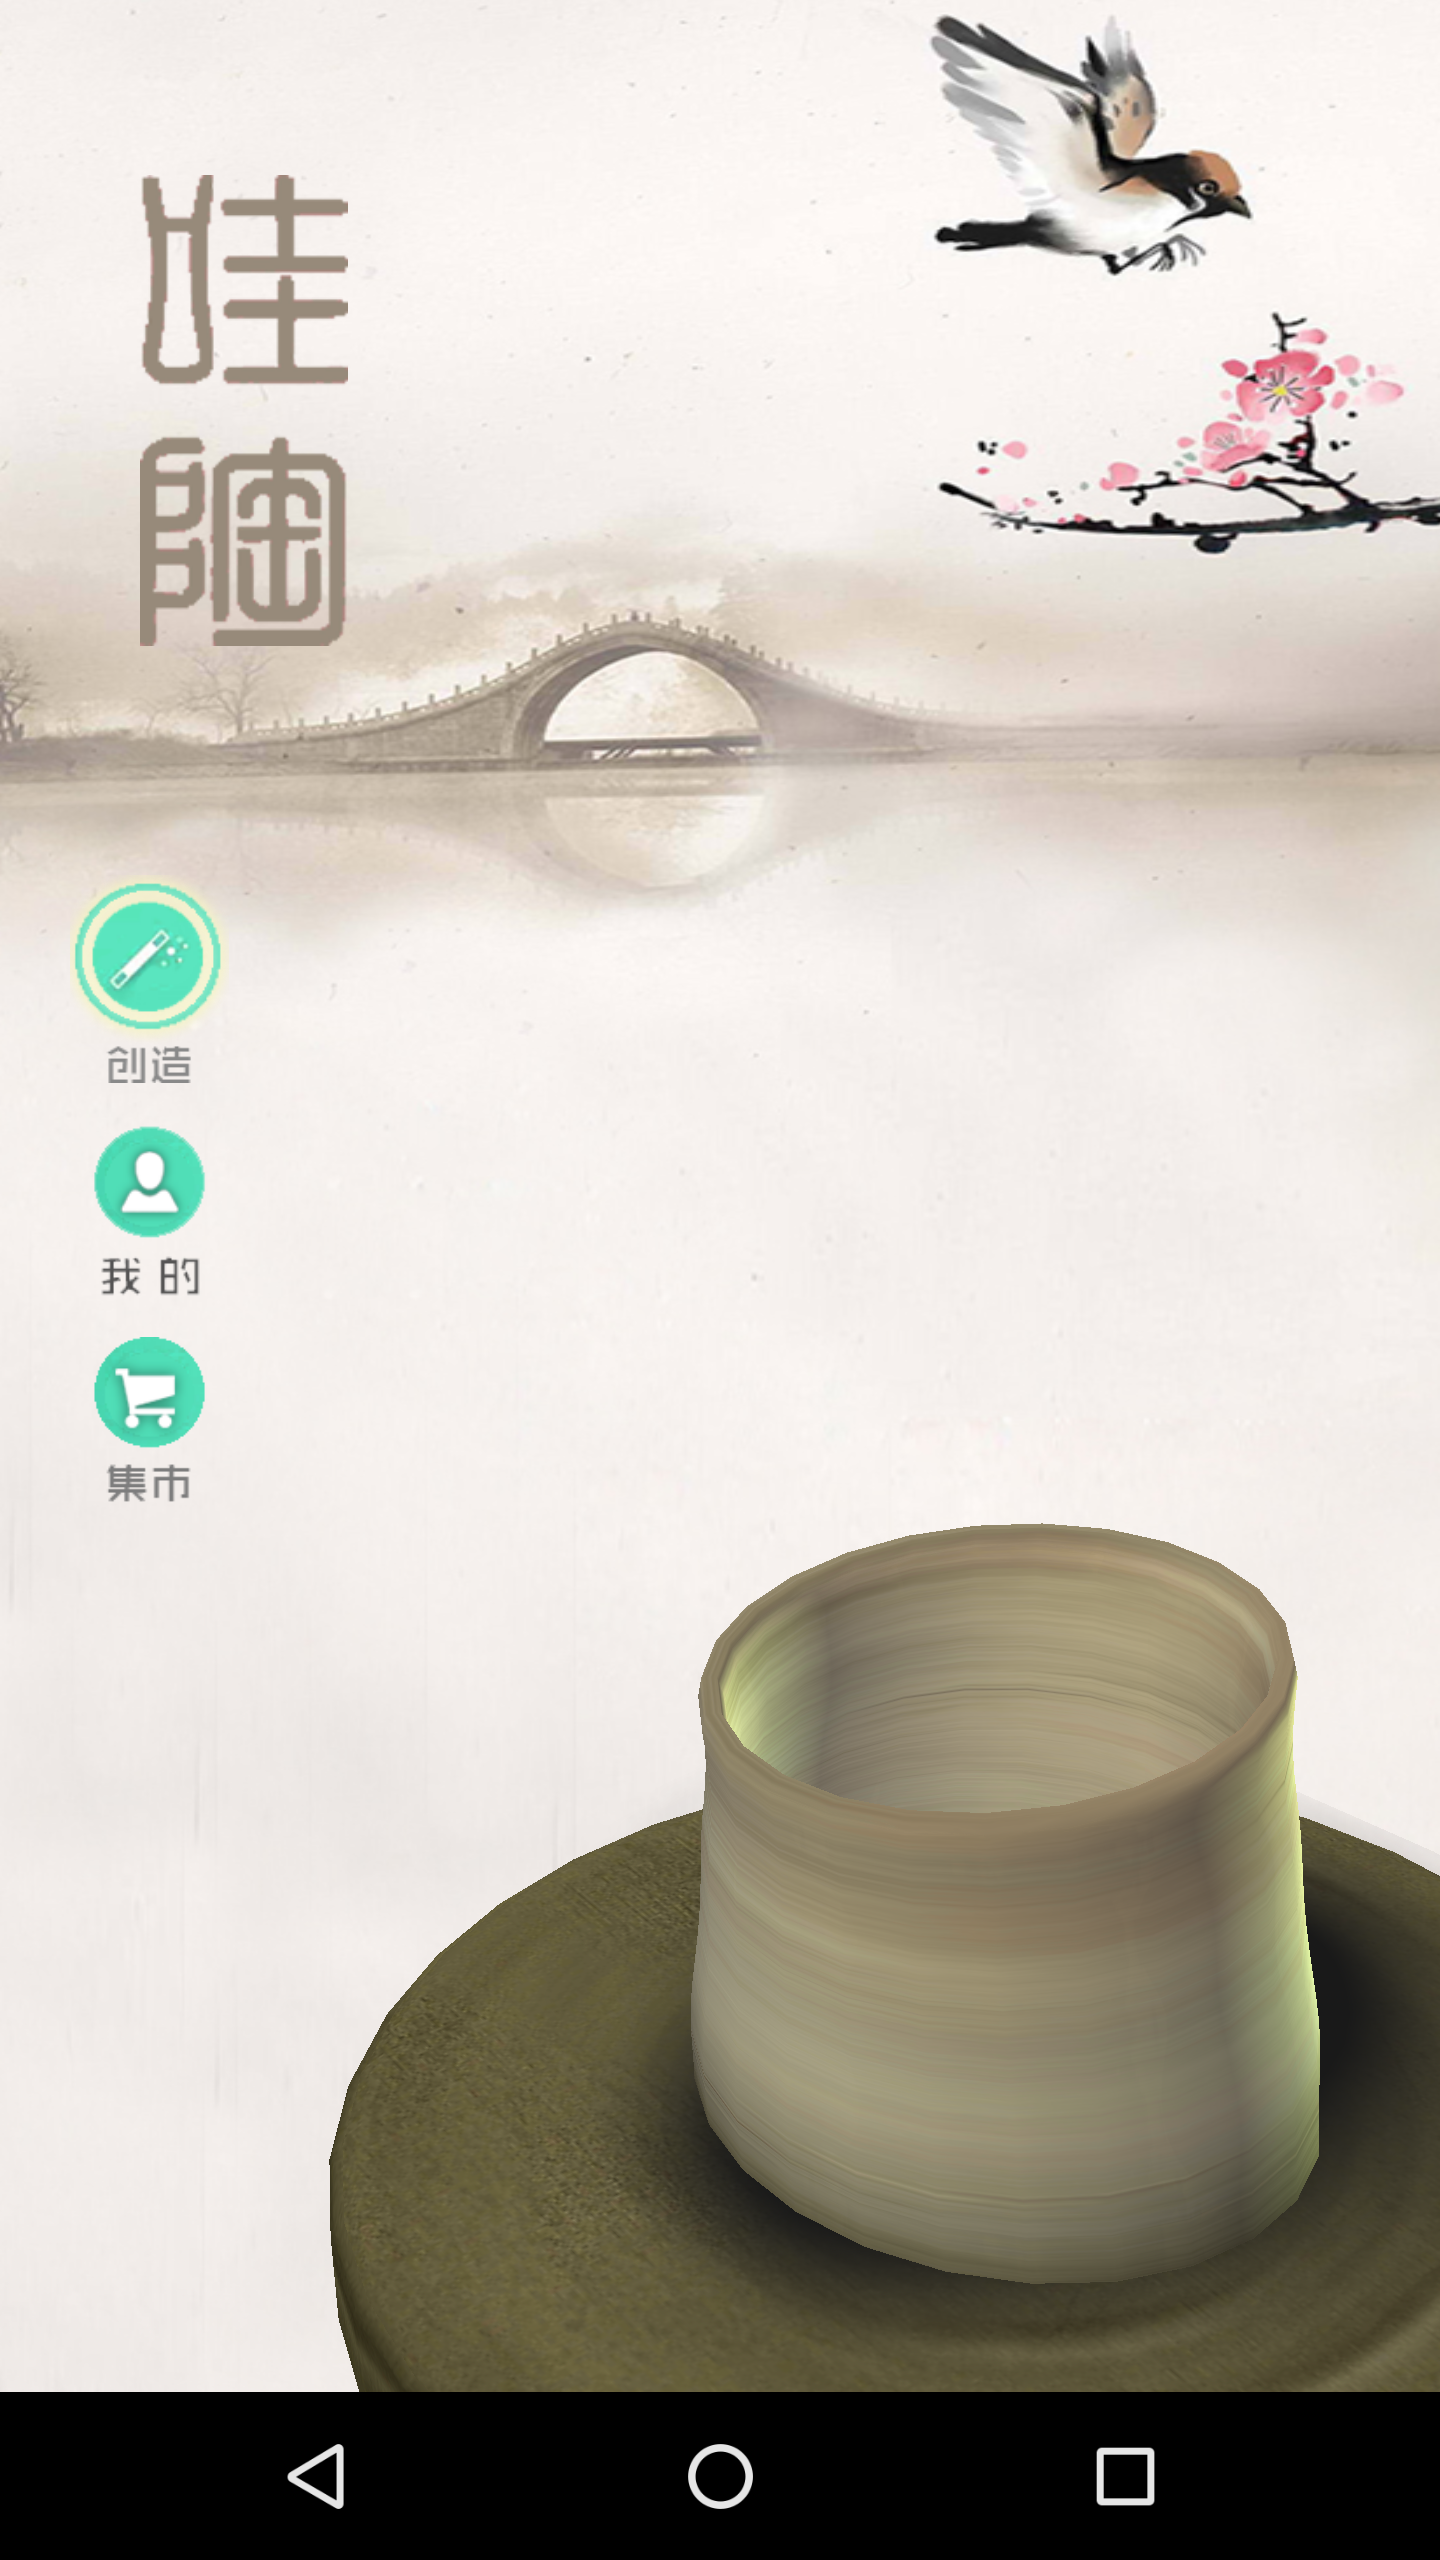
\includegraphics[width = \textwidth]{watao_0.png}
		\caption{初始界面}\label{subfig:watao_0}
	\end{subfigure}
	\begin{subfigure}[b]{.32\textwidth}
		\centering
		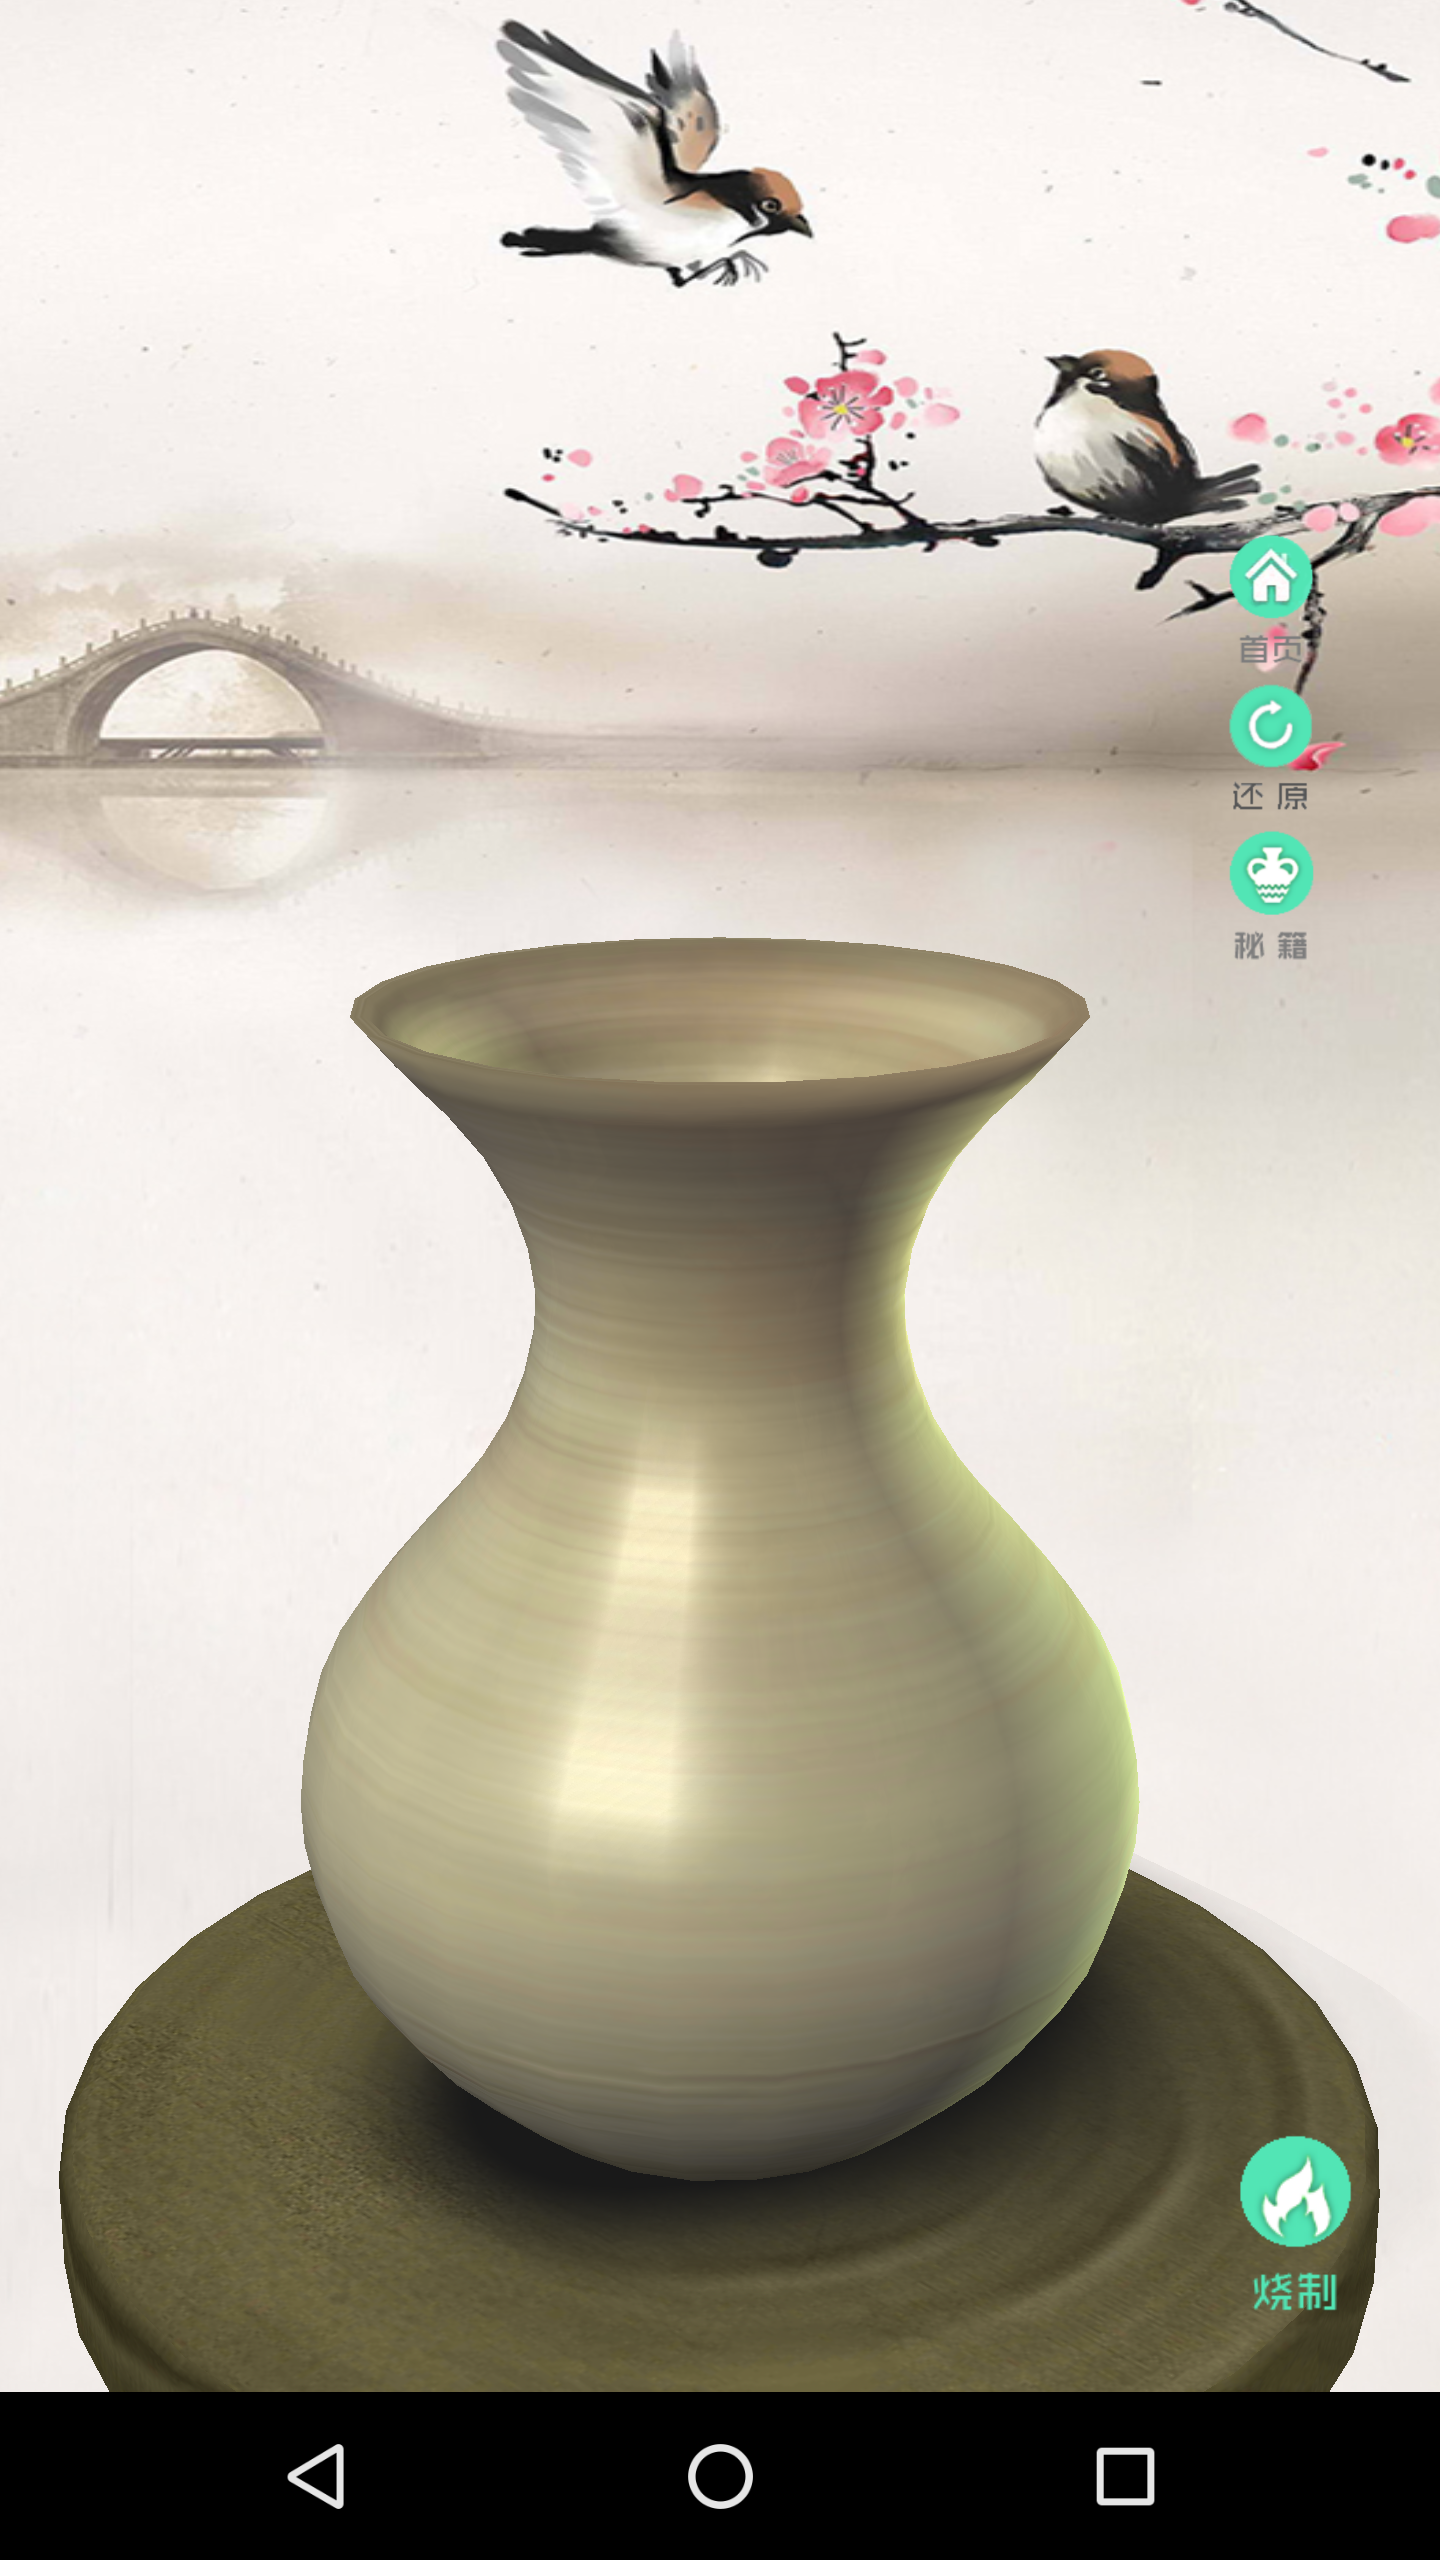
\includegraphics[width = \textwidth]{watao_1.png}
		\caption{拉胚界面}\label{subfig:watao_1}
	\end{subfigure}
	\begin{subfigure}[b]{.32\textwidth}
		\centering
		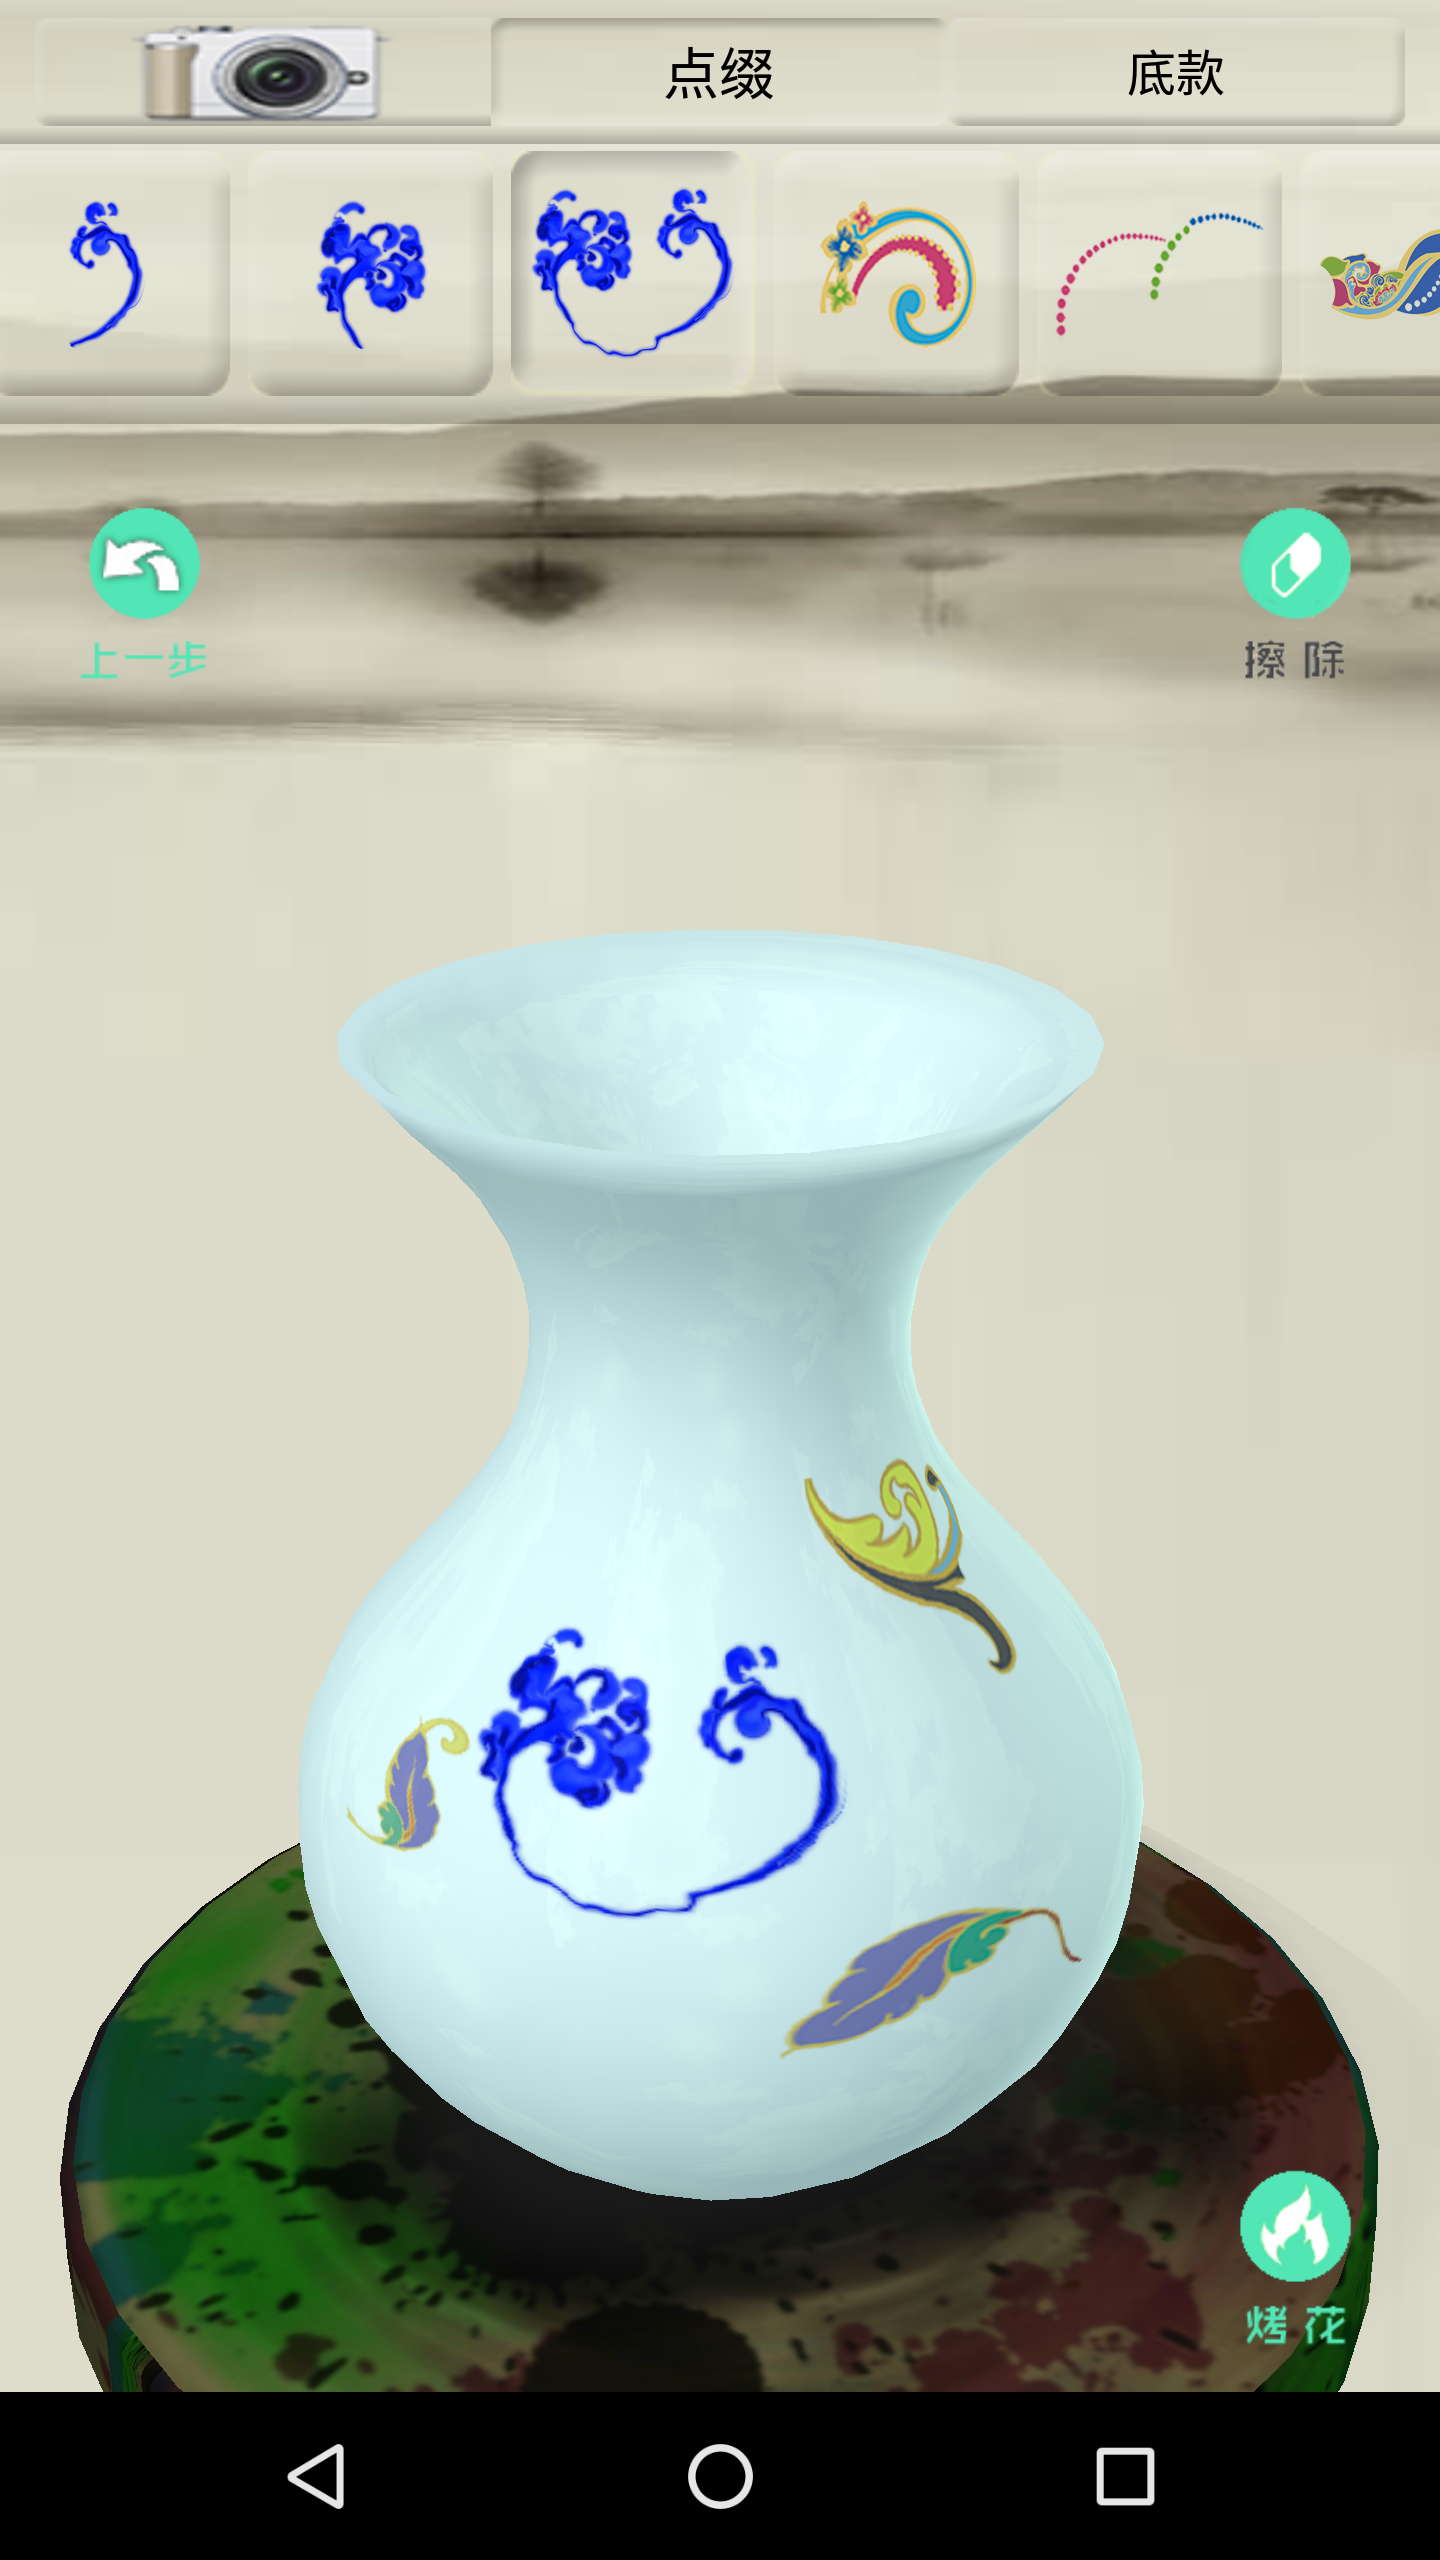
\includegraphics[width = \textwidth]{watao_2.png}
		\caption{贴图界面}\label{subfig:watao_2}
	\end{subfigure}

    \par
	\begin{subfigure}[b]{.32\textwidth}
		\centering
		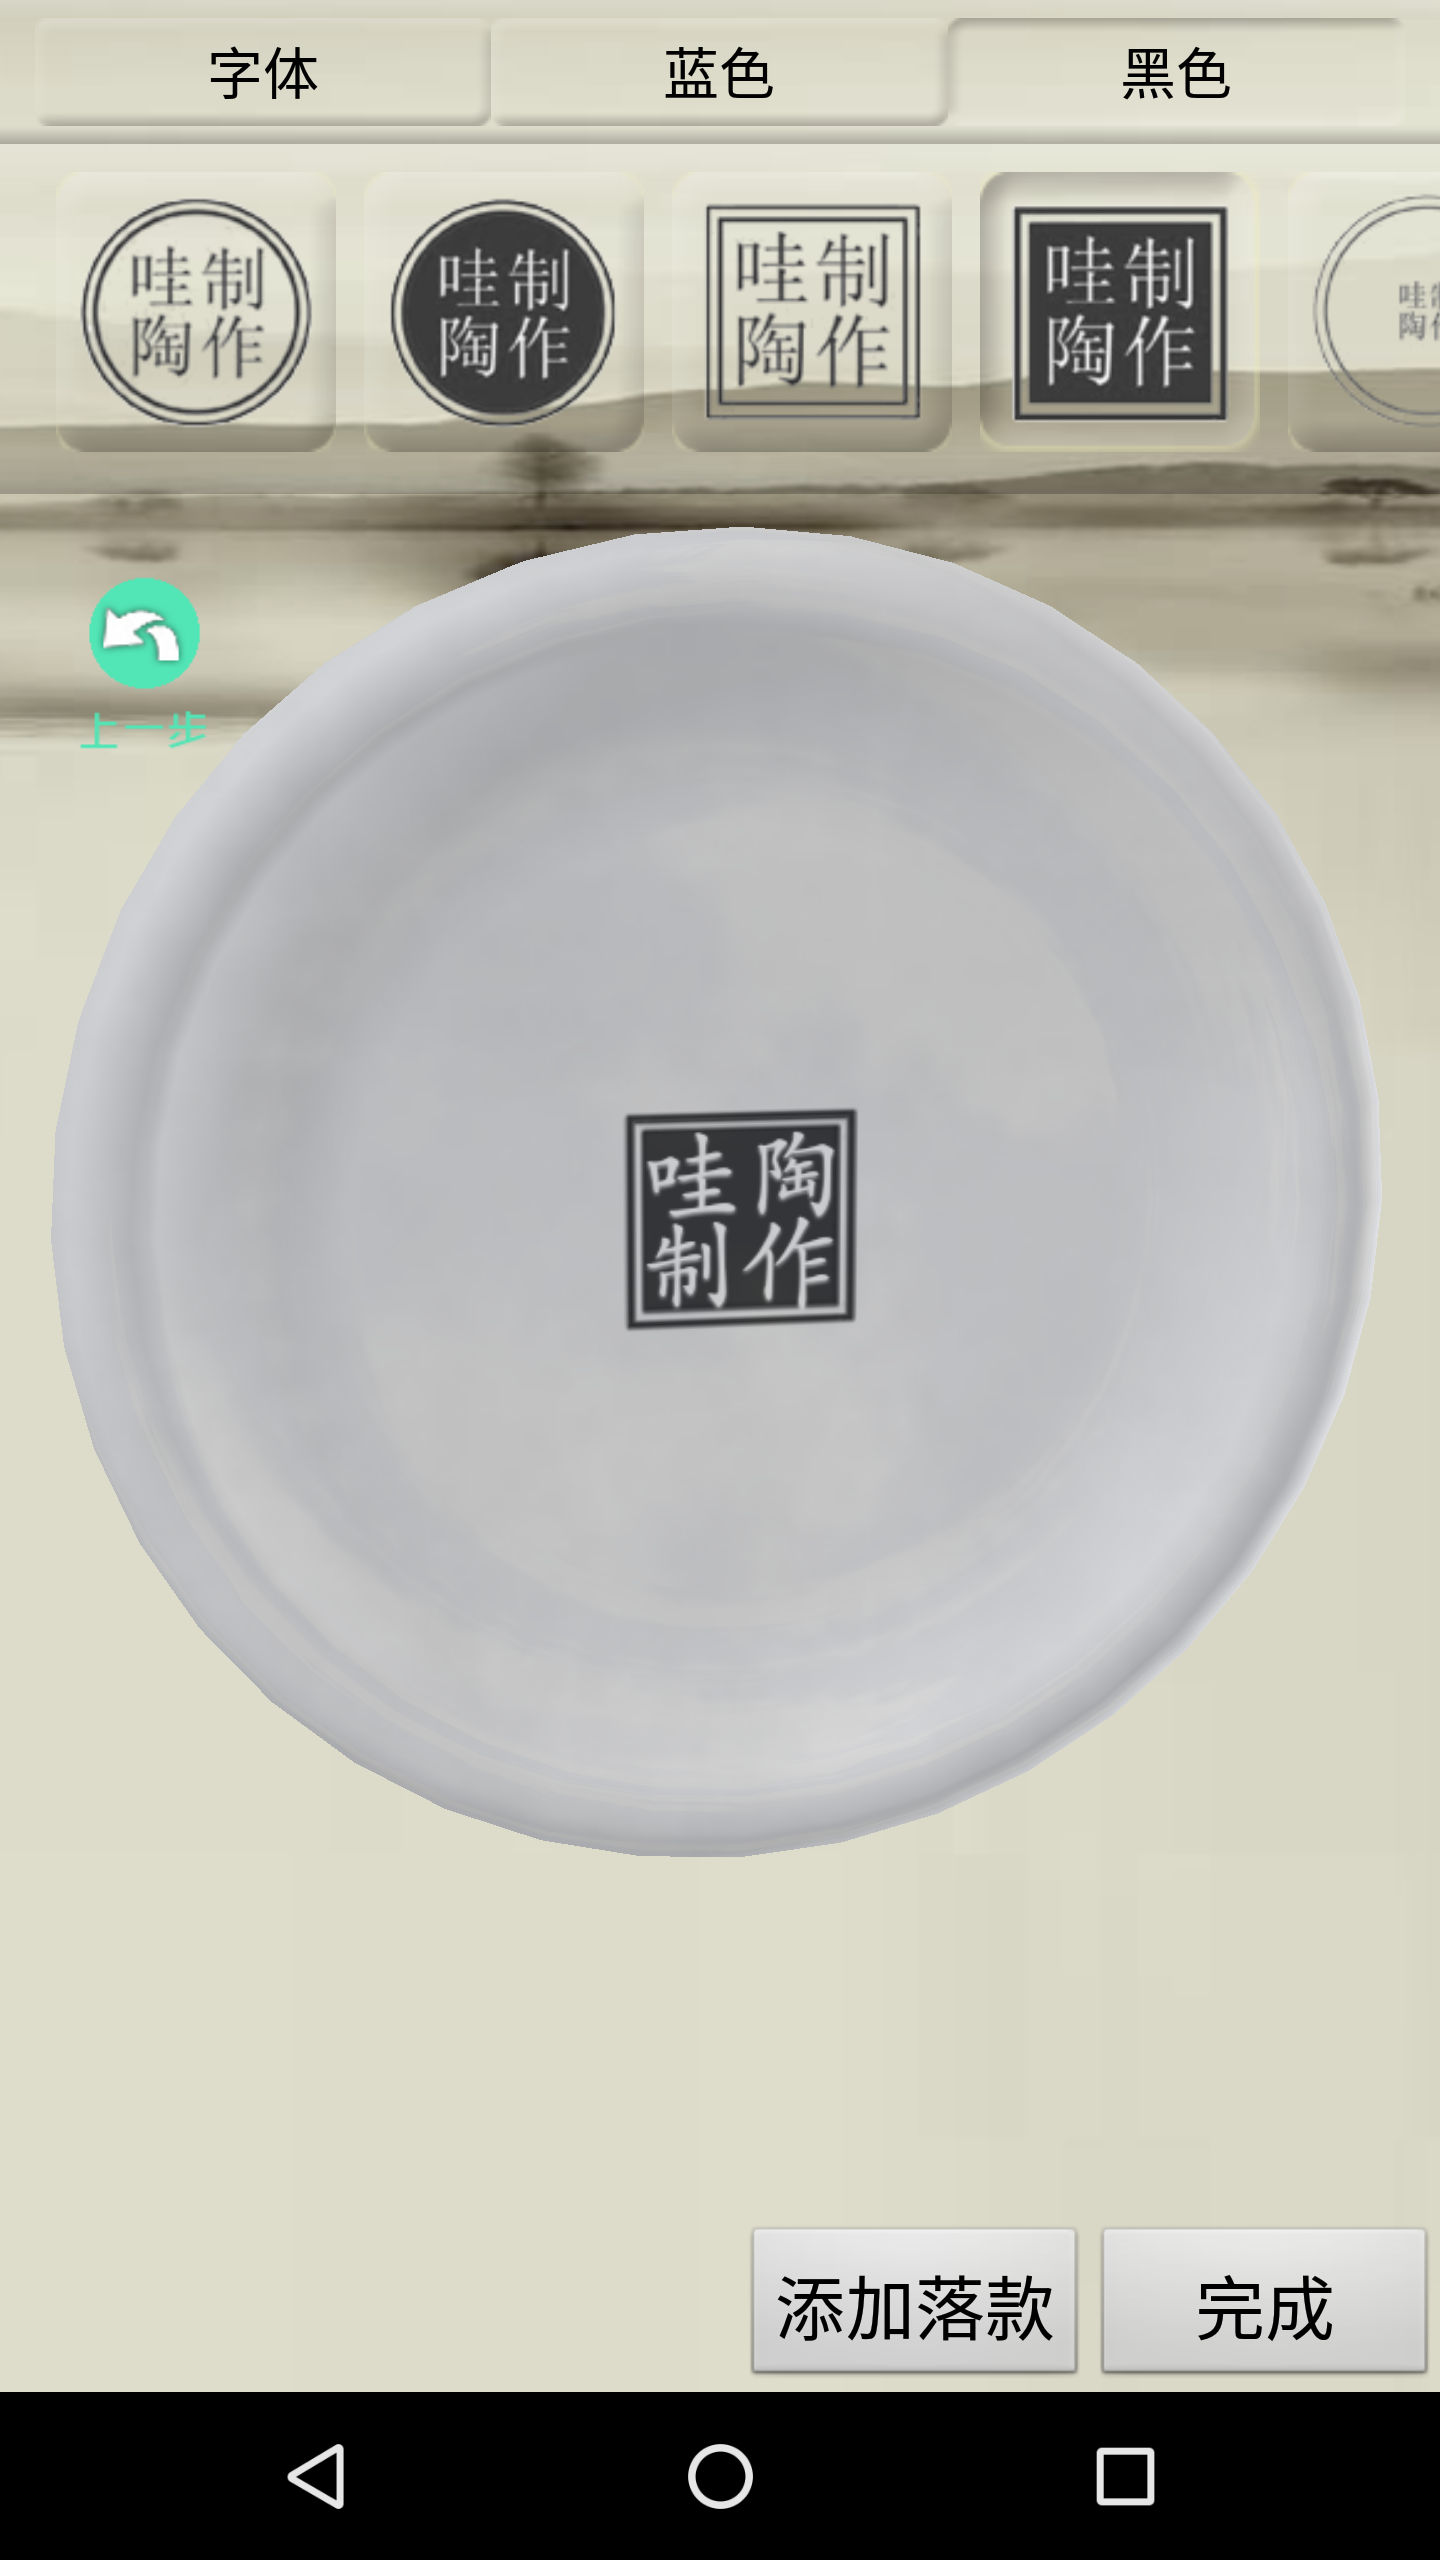
\includegraphics[width = \textwidth]{watao_3.png}
		\caption{落款界面}\label{subfig:watao_3}
	\end{subfigure}
	\begin{subfigure}[b]{.32\textwidth}
		\centering
		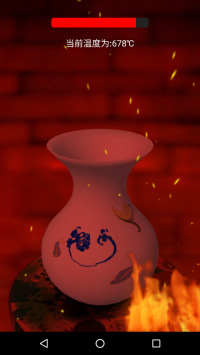
\includegraphics[width = \textwidth]{watao_4.png}
		\caption{烤花界面}\label{subfig:watao_4}
	\end{subfigure}
	\begin{subfigure}[b]{.32\textwidth}
		\centering
		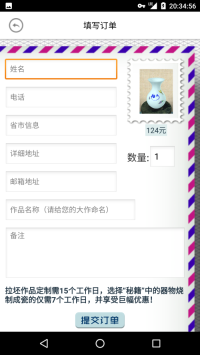
\includegraphics[width = \textwidth]{watao_5.png}
		\caption{购买界面}\label{subfig:watao_5}
	\end{subfigure}

	\caption{哇陶截图}\label{fig:watao}
\end{figure}

\section{拉胚过程的实现}

瓷器用如\autoref{fig:pottery_mesh}所示的网格模型表示,模型由内外两层网格组成,每一层网格垂直方向上有50个圆环,每个圆环由100个三角面片组成。其中\autoref{subfig:pottery_mesh_0}是初始的模型,其形状并不规则,因为我们在生成模型的时候添加了一点随机的扰动,使初始泥胚的造型更接近实际情况。\autoref{subfig:pottery_mesh_1}是用户造型后的瓷器模型。因为模型的表示较为规则,所以可以方便的将模型塑造成类似\autoref{subfig:pottery_mesh_1}那样的旋转体造型:用户手指上滑时增加模型的高度,即均匀增加垂直方向上每一层高度;用户手指水平滑动时,先根据手指点击位置计算出用户“点击”到瓷器上的点,再根据滑动幅度大小相应的调整该点所在的圆环及邻近圆环的半径,以达到改变瓷器器身粗细的目的。离用户点击位置越远的圆环变化幅度越小。该过程如\autoref{fig:shape}所示,

\begin{figure}[htbp]
	\centering
	\begin{subfigure}[b]{.4\textwidth}
		\centering
	    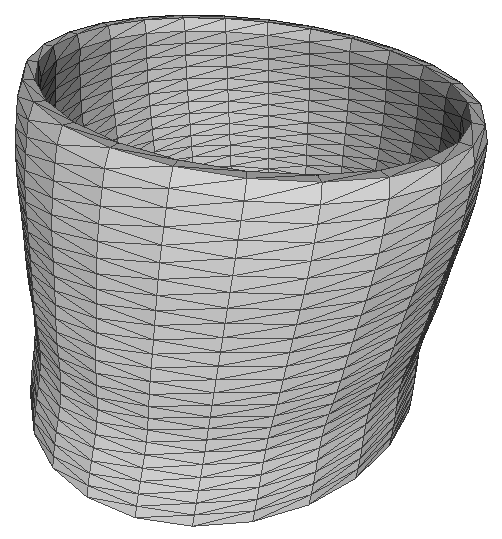
\includegraphics[width = \textwidth]{pottery_mesh_0.png}
		\caption{初始瓷器网格模型}\label{subfig:pottery_mesh_0}
	\end{subfigure}
	\begin{subfigure}[b]{.4\textwidth}
		\centering
		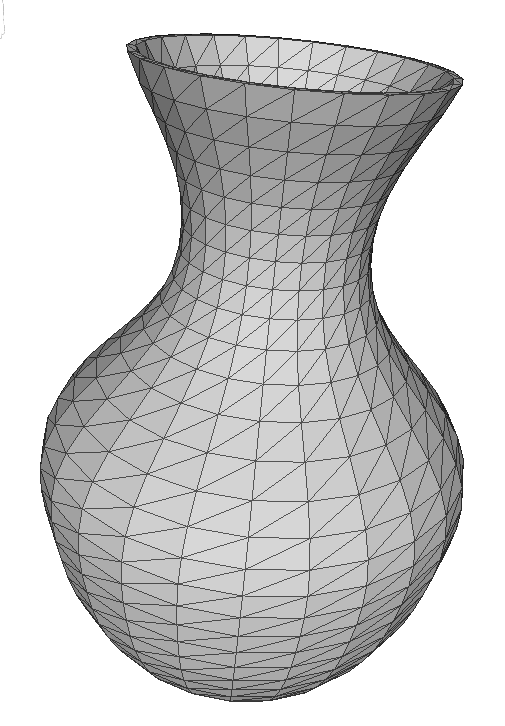
\includegraphics[width = \textwidth]{pottery_mesh_1.png}
		\caption{拉胚后瓷器网格模型}\label{subfig:pottery_mesh_1}
	\end{subfigure}
	\caption{瓷器网格模型}\label{fig:pottery_mesh}
\end{figure}

\begin{figure}[htbp]
	\centering
	\begin{subfigure}[b]{.4\textwidth}
		\centering
	    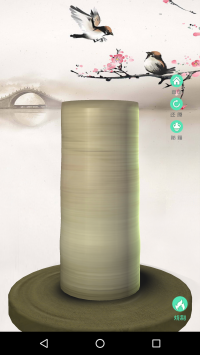
\includegraphics[width = \textwidth]{shape_0.png}
		\caption{水平拉胚之前}\label{subfig:shape_0}
	\end{subfigure}
	\begin{subfigure}[b]{.4\textwidth}
		\centering
		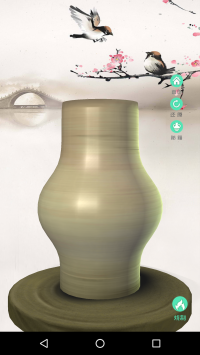
\includegraphics[width = \textwidth]{shape_1.png}
		\caption{一次水平拉胚之后}\label{subfig:shape_1}
	\end{subfigure}
	\caption{拉胚过程}\label{fig:shape}
\end{figure}

在真实的陶瓷制作过程中,泥胚塑形阶段,制作陶瓷的工匠不仅可以通过转台将瓷器拉成一个完全对称的旋转体,如\autoref{subfig:pottery_shape_0}所示,还可以通过手工捏胚将瓷器塑造成更具创造性的形状,但是上方描述的方法只提供两个自由度,只能将模型塑造成旋转体,可以模拟通过转台拉胚,但是无法模拟捏胚过程。所以我们将本文的自由变形算法引入到了哇陶中来模拟手工捏胚过程,以帮助用户得到满意的造型。

\begin{figure}[htbp]
	\centering
	\begin{subfigure}[b]{.4\textwidth}
		\centering
		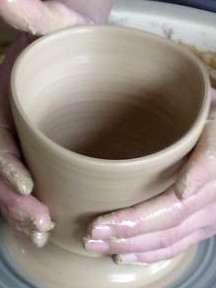
\includegraphics[width = \textwidth]{pottery_shape_0.jpg}
		\caption{转盘拉胚}\label{subfig:pottery_shape_0}
	\end{subfigure}
	\begin{subfigure}[b]{.4\textwidth}
		\centering
		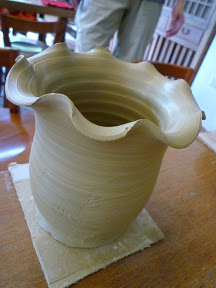
\includegraphics[width = \textwidth]{pottery_shape_1.jpg}
		\caption{莲花口}\label{subfig:pottery_shape_1}
	\end{subfigure}
	\caption{泥胚塑形}\label{fig:pottery_shape}
\end{figure}

\section{改进拉胚交互}
在哇陶中实现我们的自由变形算法时,我们发现用户交互十分不方便。由于安桌手机没有鼠标键盘,其主要交互手段为触控,且手机屏幕相对于桌面显示器要小很多。所以本文方法的交互方式\footnote{本文方法需要先选定控制顶点,然后通过位移控制顶点来变形模型。}并不适合手机用户,尤其是的选定控制顶点的阶段,用户因为手机屏幕小,手指点击精度低,而以体为变形空间的自由变形方法均存在控制顶点数目过多的现象,所以用户很难快速准确的选定控制顶点。

为了解决这一问题,本文采用了直接自由变形\cite{hsu1992}以改善交互。直接自由变形允许用户指定模型中某些点变形后的空间位置,然后以这些点变形前后的位移为约束,以最小化控制顶点的位移为优化目标,用约束优化方法反求出所有控制顶点的位移。再以新的控制顶点变形整个模型。在该方法中,用户输入的位移与模型的变形在着较为明确的对应关系,使得自由变形算法更为简单易用。最为关键的是该方法无需在变形之前选择控制顶点,正好弥补了本文方法在移动设备中选点所产生的交互问题。

并且我们观察到,用户比较倾向于捏制一些对称的器型。所以我们还在直接自由变形的基础了提供了“对称变形”的功能。如用户指定模型上的点$P$变形前后的位移是$V$,$P$的空间位置是$(P_x, P_y, P_z)$,向量$V$为$(V_x, V_y, V_z)$。那么我们可以将$P$,$V$做一个关于$Y$\footnote{$Y$轴即为瓷器从底部到顶部的方向}轴的中心对称。得到$V'$和$P'$分别为$(-P_x, P_y, -P_z)$,$(-V_x, V_y, -V_z)$。这样我们就可以以$P$,$P'$的位置和位移为输入进行直接自由变形,以得到对称的变形结果。用户还可以选择多生成几个对称的点,以生成更加繁复的对称图案。如\autoref{fig:dffd}所示

\begin{figure}[htbp]
	\centering
	\begin{subfigure}[b]{.4\textwidth}
		\centering
		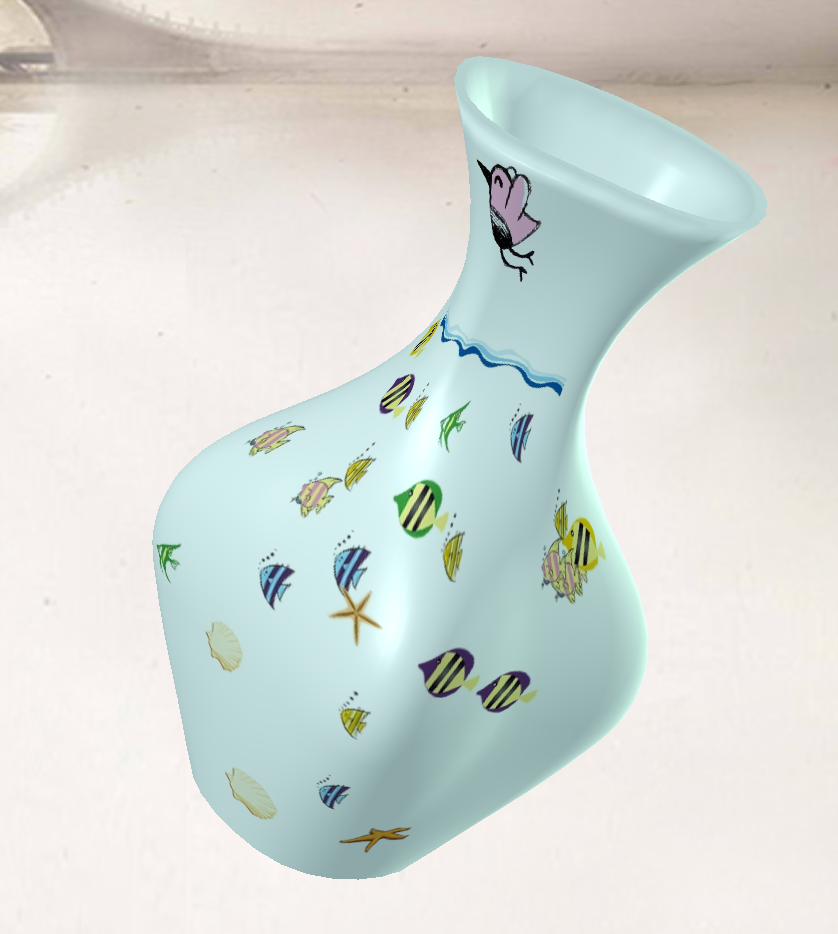
\includegraphics[width = \textwidth]{dffd_0}
		\caption{对称点数目为3}\label{subfig:dffd_0}
	\end{subfigure}
	\begin{subfigure}[b]{.4\textwidth}
		\centering
		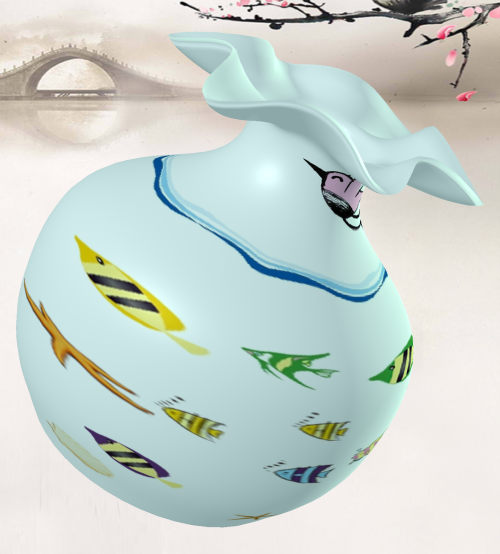
\includegraphics[width = \textwidth]{dffd_1}
		\caption{对称点数目为4}\label{subfig:dffd_1}
	\end{subfigure}
	\caption{对称变形结果}\label{fig:dffd}
\end{figure}
